

\chapter{Softwarearchitektur der bestehenden Software}

    Analysemethoden der Informatik für Software sind in der Regel für die verschiedenen Design-Phasen einer Software entwickelt worden.
    Eine von mir durchgeführte Recherche ergab, dass sich Analyse-Tools und Methoden für bestehende Software vor
    allem darauf fokussieren die Performance, Speichermanagement und Benutzererfahrung zu bewerten.
    Die Architektur einer Software spielt dabei eine untergeordnete Rolle.
    Für die Neuentwicklung der bestehenden Software wird allerdings im Folgenden die Programmstruktur dargestellt und analysiert.
    Die Performance der Software und ihr Speicherverbrauch spielen für die $\mu$Plant eine untergeordnete Rolle.
    Eine Bewertung der Programmkomponenten sollte also anhand folgender Kriterien bewertet werden:

    \begin{itemize}
        \item Ihrem Nutzen für den Anwender
        \item Zuverlässigkeit
        \item Umgang mit erwartbaren Fehlern
    \end{itemize}

    Der Programmcode sollte zudem
    \begin{itemize}
        \item Leicht lesbar und verständlich
        \item Zuverlässig und robust
        \item gut erweiterbar sein.
    \end{itemize}

    \\
    In einem C\# Projekt sind UI und Logik in getrennten Dateien implementiert.
    XAML Dateien sind eine angepasste Form von XML-Dateien und legen somit fest wie das GUI gerendert wird.
    XAML.CS Dateien enthalten die dahinterliegende Logik inklusive Schnittstellen zu anderen Programmteilen.
    Am Beispiel des Startbildschirms des Programms \glqq Lagerverwaltung 3.0\grqq wird der grundlegende Programmaufbau geschildert.
    Im Weiteren wird wegen der Komplexität und des fehlenden Mehrwerts darauf verzichtet.
    Ich verzichte aus den gleichen Gründen auf die detaillierte Funktionsweise der grafischen ELemente und der Events
    sowie ihrer Eventhandler.
    \\
    In den erstellen Klassendiagrammen ist gut ersichtlich, welche Klasse Events nutzt.
    Die Klasse \verb|INotifyPropertyChanged| stellt die benötigten Listeners dafür bereit und wird an andere Klassen vererbt.

    \subsection {Lagerverwaltung 3.0}

    Wie in dem einleitenden Abschnitt angekündigt wird zunächst der grundlegende Aufbau des Programms aufgelistet.
    \\
    Die Datei \verb|App.xaml| ist der Einstiegspunkt des Programms.
    In ihr wird ein Objekt der Application-Klasse mit allen benötigten Ressourcen erzeugt.
    Als Start URL ist \verb|MainWindow.xaml| angeben.
    \\
    In der Datei ist beschrieben wie der Startbildschirm gerendert wird.
    Zunächst wird ein Banner gerendert, bestehend aus dem Titel des Programms, dem Logo des Instituts und der $\mu$Plant
    (Siehe Abb. 2.1 Bereich \glqq A\grqq).
    Es werden außerdem alle benötigten Datenobjekte erzeugt.
    Sie lassen sich wie folgt einteilen:
    \\
    \begin{itemize}
        \item Objekte und Variablen, die dem Lager zugeordnet sind:
            \begin{itemize}
                \item Ein Objekt \verb|inventory| der Klasse \verb|Inventory| für das Inventar mit \verb|null| initialisiert.
                \item Ein Objekt \verb|storageMatrix| von der Klasse \verb|PalletMatrix| erzeugt.
                \item Ein Object \verb|commissionMatrix| von der Klasse \verb|PalletMatrix| erzeugt.
                \item Ein Objekt \verb|mobileRobot| von der Klasse \verb |MobileRobot| erzeugt.
                \item Außerdem eine Variable \verb|lastCupRead| vom Datentyp \verb|ushort| (16-Bit-Ganzzahl, vorzeichenlos) mit 0 initialisiert.
            \end{itemize}
            \item Objekte und Variablen initialisiert, die dem ABB Controller zugeordnet sind:
            \begin{itemize}
                \item Ein Objekt \verb|commands| von der Klasse \verb|controllerCommandList|.
                \item Ein Objekt \verb|controllerProperties| von der Klasse \verb|RobotControllerProperties|.
                \item Ein Objekt \verb|controllerBase| von der Klasse \verb|RobotControllerBas|, mit dem Initialisierungswert \verb|null|.
                \item Ein Objekt \verb|controllerSim| von der Klasse \verb|RobotSimulator|.
            \end{itemize}
    \end{itemize}
    Im Constructor der Klasse \verb|MainWindow| werden zudem der ModBus und der Roboter Controller initialisiert
    und gerendert (Abb. 2.1 Bereiche \glqq B\grqq und \glqq C\grqq).
    Die Produktliste wird aus der Datei \verb|Produkte.db| geladen und gerendert (Abb. 2.1 Bereich \glqq D\grqq).
    Daten des Lagers und des mobilen Roboters sowie die Kommissionsdaten werden aus der Datei \verb|CommissionData.db|
    geladen und anschließend das Inventar gerendert:
    Es wird einerseits eine Produktliste im Bereich \glqq E\grqq in Abb. 2.1 erzeugt, die um die gelagerte Menge ergänzt ist.
    Produkte ohne Lagermenge können mit einer Checkbox wahlweise ein- und ausgeblendet werden.
    Andererseits werden die Daten genutzt, um im Bereich \glqq G\grqq der Abbildung das Lager zu visualisieren.
    Die drei Reihen \glqq TOP\grqq, \glqq MIDDLE\grqq und \glqq BOTTOM\grqq solen die drei Regalböden des Lagerregals nachbilden.
    Die Slots A1\ldots A6, H1\ldots H6 sowie H7\ldots H12 sind die Plätze für je eine Palette, die wiederum Platz für
    je zwei Becher hat.
    Der Ursprung dieser Bezeichnung konnte während der Vorbereitungen auf diese Arbeit nicht geklärt werden.
    Das reale Pendant ist mit L1\ldots L18 gekennzeichnet.
    \\
    Im Bereich \glqq F\grqq werden alle Ereignisse der Software als text angezeigt.
    Das können Fehler sein aber auch Fortschritte im Programmablauf.
    \\
    Im mittleren Bereich ist die Anordnung von Roboter, Andockstation und Kommissioniertisch symbolisiert.
    Der \glqq Start\grqq -Knopf startet den Automatikbetrieb.
    Wenn keine Verbindung zum Modbus hergestellt werden kann, wird dem Benutzer angeboten die Vorgänge zu simulieren.
    m Klassendiagramm Abb. 2.2 wird jedoch schnell deutlich, dass dieser Simulationsbetrieb nicht dazu genutzt werden
    kann, um etwaige Fehler zu erkennen, da dazu eine ganz andere Klasse verwendet wird.
    Im Bereich \glqq Mobile Robot\grqq wird nach erfolgreichem Andocken das erkannte Produkt angezeigt.
    Dem Bediener wird hier angeboten die Daten manuell zu manipulieren oder Details auszublenden.
    Im Bereich \glqq Workbench\grqq werden bis zu zwei Paletten mit ihrem Inhalt gerendert.
    Auch hier wird dem Benutzer angeboten, die Daten per Hand zu manipulieren.

    \begin{figure}[h]
        \label{fig:figure}
        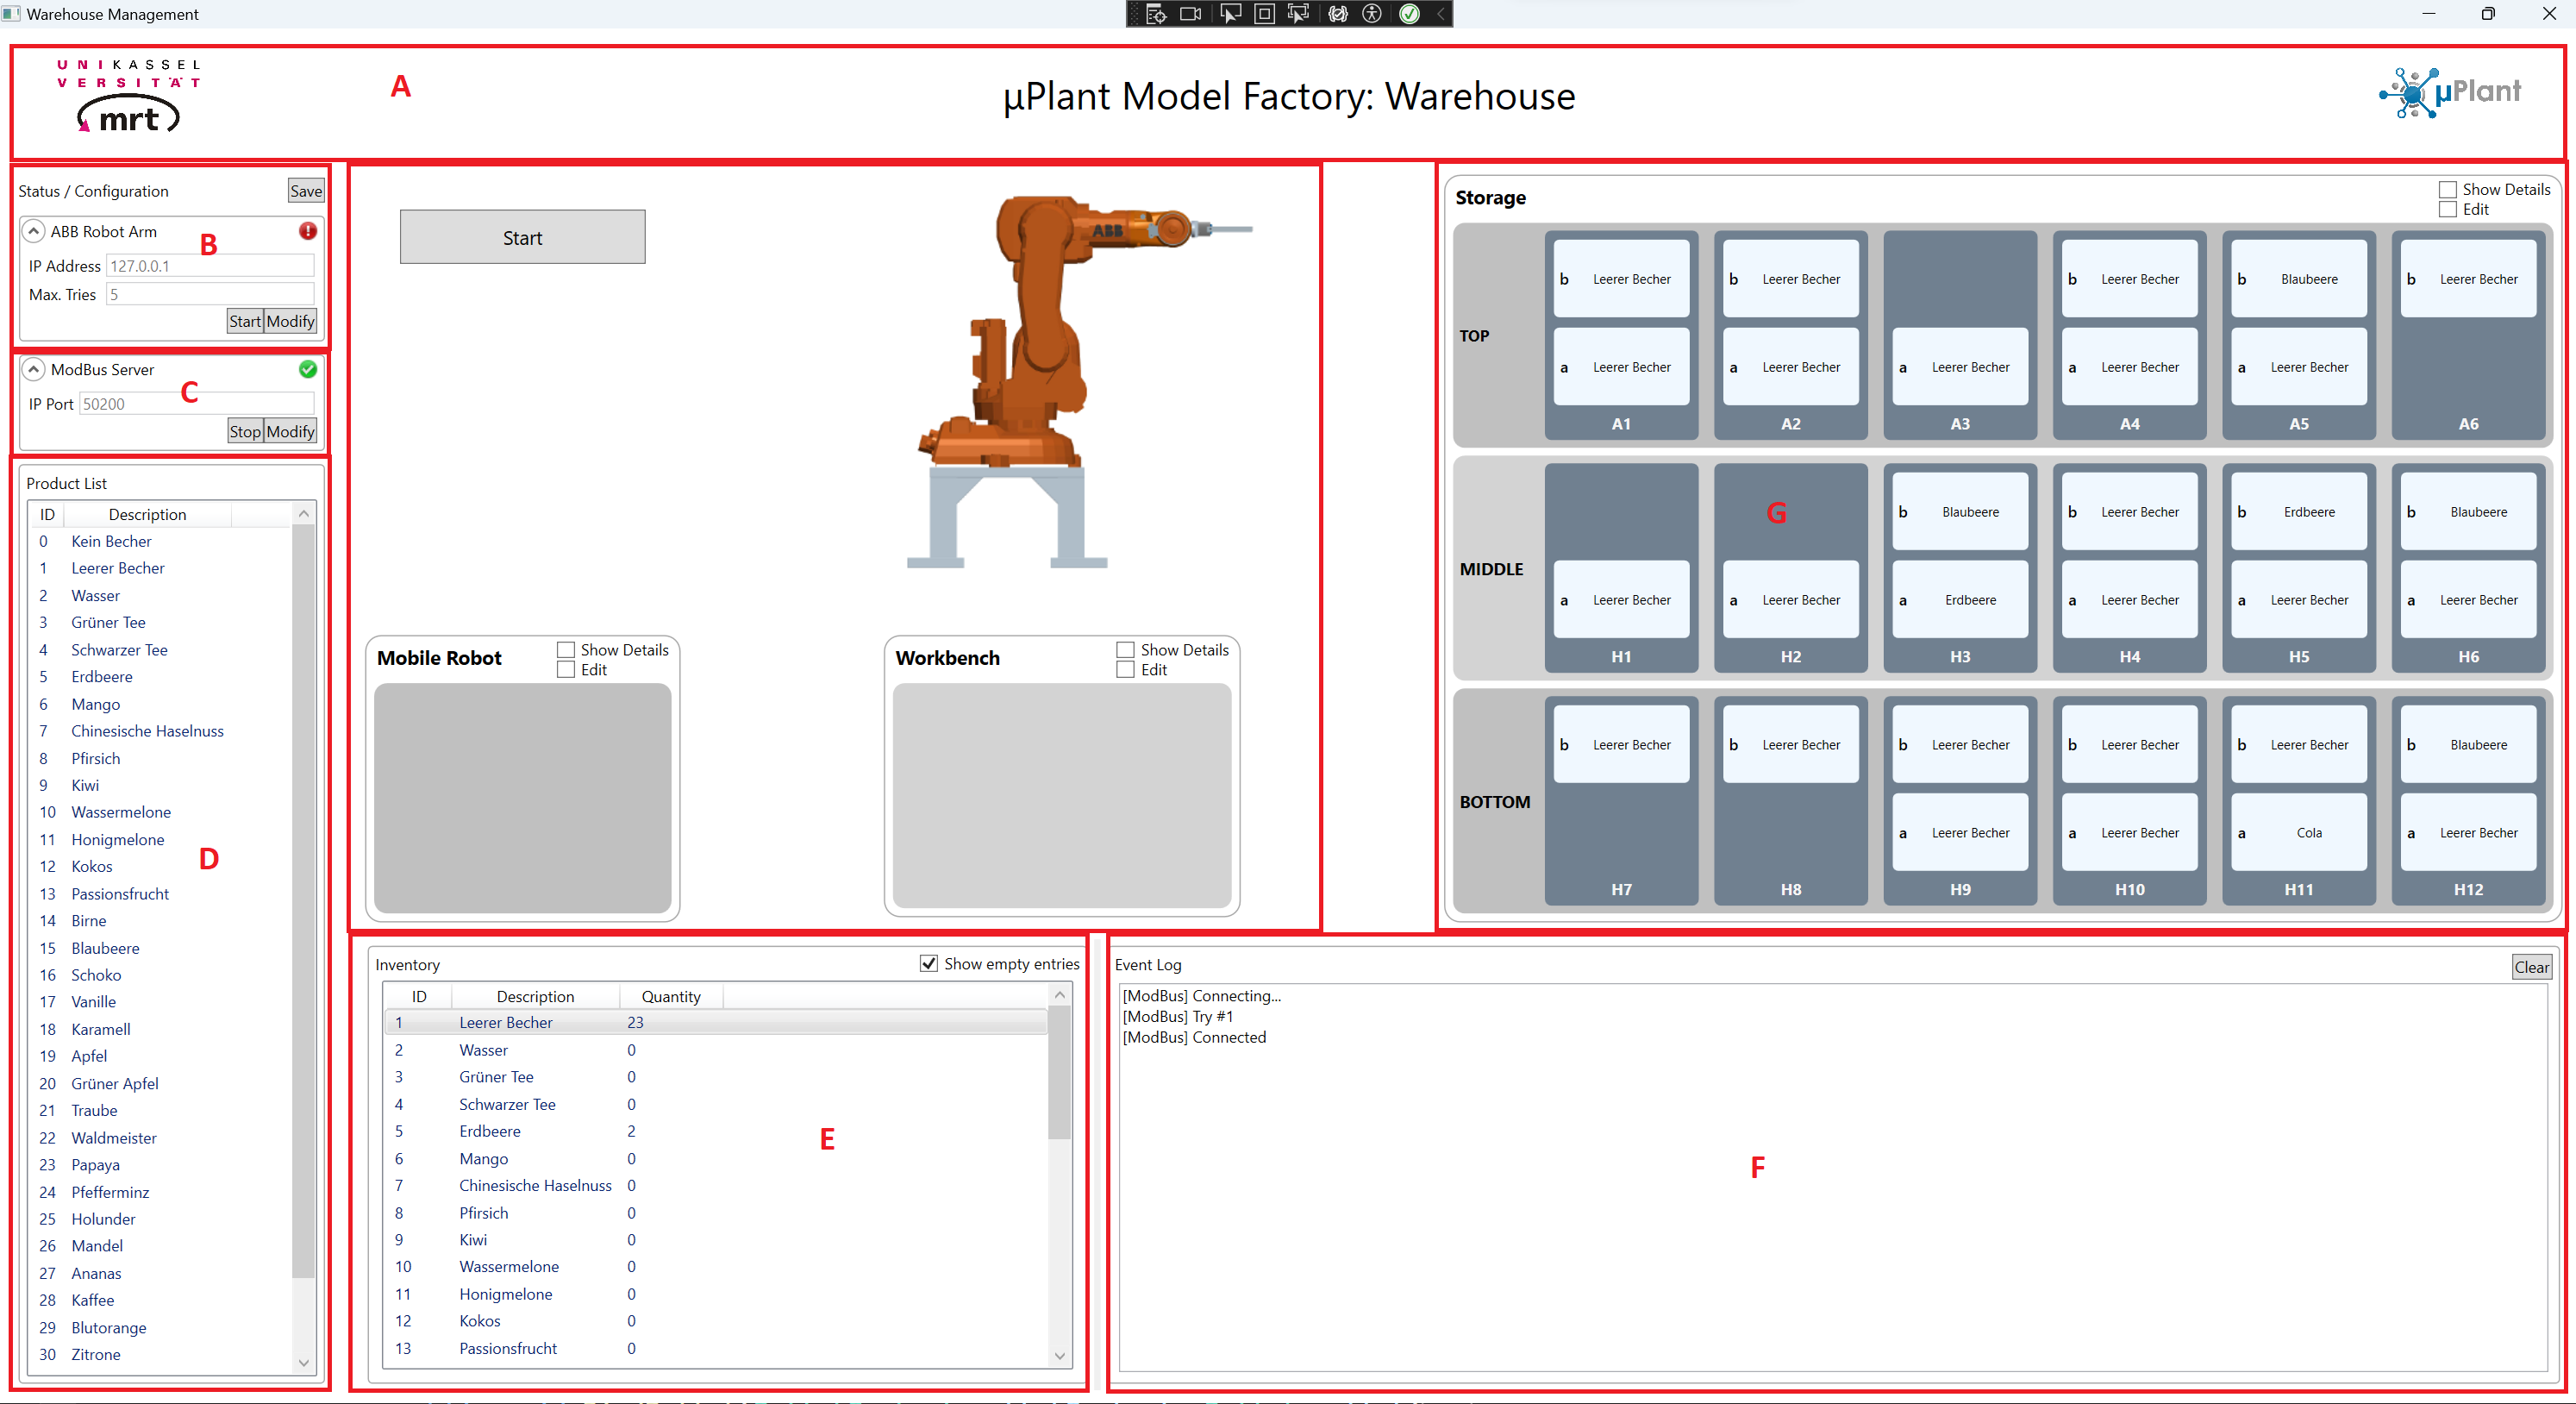
\includegraphics[width = \textwidth ]{Bilder/LV_Startbildschirm}

        \caption[Ansicht des Startbildschirms]
        {\small Startbildschirm der Anwendung, zur besseren Beschreibung sind die Bedienbereiche rot umrandet und mit
        Buchstanben gekennzeichnet}
        \centering
    \end{figure}

    \subsubsection{Datenstruktur}

    Die bestehende Software dient dazu Lagerpakete vom mobilen Roboter auf die Werkbank oder ins Lager zu bewegen.
    Oder alle möglichen Kombinationen davon.
    Das Konzept der $\mu$Plant beschränkt sich dabei auf eine Palette, die so ausgeführt ist, dass der Greifer des
    Industrieroboters sie sicher bewegen kann.
    Im Wesentlichen ist es ein Quader mit zwei seitlichen Längsnuten.
    Eine Palette enthält zwei senkrechte Bohrungen, die es ermöglichen je einen Becher aufzunehmen.
    Ein Becher ist ein transparentes, zylindrisches Gefäß aus Acrylglas mit einem Absatz, der etwa mittig in der
    Höhe angebracht ist, sodass der Greifer die Becher einzeln bewegen kann.
    Es wird also immer entweder
    \begin{itemize}
        \item Eine Palette
        \item Ein Becher
        \item eine Palette mit einem oder mehreren Bechern
    \end{itemize}
    bewegt.
    Der Programmierer hat sich diese Struktur angeeignet und in der Datenmodellierung umgesetzt.
    In Abb. 2.2 ist gut ersichtlich, dass die Klasse \verb|StorageElementBase| an die Klassen \verb|Cup| und \verb|Pallet|
    vererbt (schmale Linie mit leerem Pfeil, in Anlehnung an UML). Eigenschaften, die sowohl Palette als auch den
    Becher betreffen sind in dieser Klasse implementiert.
    Weiterhin findet sich das Lager als eigene Klasse \verb|Inventory| und der mobile Roboter als \verb|MobileRobot| wieder.
    Die \verb|Inventory|-Klasse ist jedoch nicht das Lager im Sinne von Abb 2.1 Bereich \glqq G\grqq, sondern auf die Liste in
    Bereich \glqq E\grqq.
    Ansonsten versucht das Datenmodell nicht weiter reale Prozesse im Programm abzubilden.
    \\
    \begin{figure}[ht]
        \label{fig:figure2}
        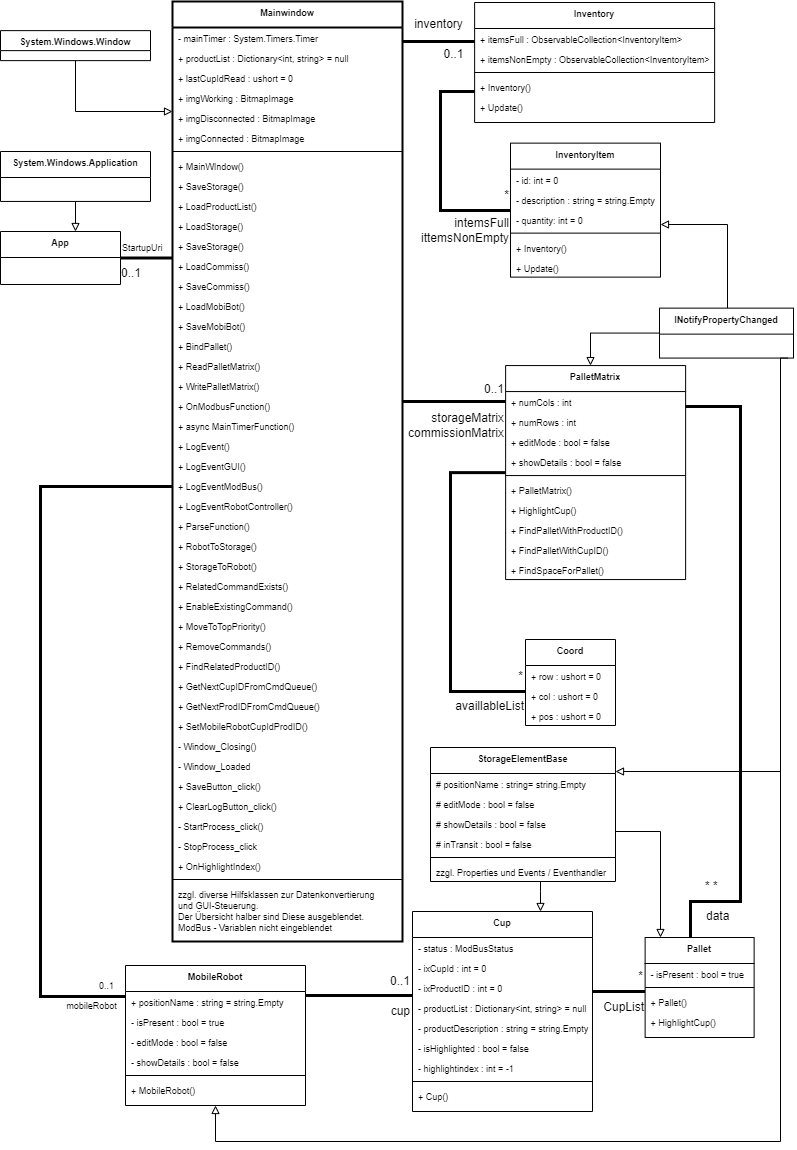
\includegraphics[width = \textwidth ]{Bilder/LV_Klassendiagramm_Datenmodell}
        \caption[Klassendiagramm Datenmodells ]
        {\small Klassendiagramm der MainWindow-Klasse mit vererbenden- und Datenmodell - Klassen }
        \centering
    \end{figure}

    Zentrales Element ist die \verb|MainWindow| Klasse.
    Sie implementiert eigentlich eine Interface-Klasse \verb|System.Windows.Window| und ist somit als GUI Element gedacht.
    Der Programmierer hat sie allerdings als Daten-Hub verwendet.
    Wie oben geschildert werden beim Rendern des Fensters alle benötigten Datenobjekte erzeugt oder aus Dateien geladen.
    \begin{itemize}
        \item In der Klasse \verb|Inventory| wird der Inhalt der Datei \verb|Produkte.db| in zwei Listen geladen, sodass
        eine Liste mit lagernden Produkten und eine vollständige Produktliste gespeichert werden.
        Eine Instanz \verb|inventory| wird zur Laufzeit erzeugt. Wenn die Dateien \verb|Produkte.db| und
        \verb|StorageData.db|zu dem Zeitpunkt nicht verfügbar ist, stürzt das Programm ab.
        \item In der Klasse \verb|PalletMatrix| wird die Datei \verb|StorageData.db| bzw. \verb|CommissionData.db|
        geladen um einen zweidimensionalen Array \verb|data| zu erzeugen.
        Jedes Array-Element ist ein Objekt der Klasse \verb|Pallet| und enthält eine Liste \verb|CupList| von Objekten
        der Klasse \verb|Cup|.
        Diese Struktur wird dazu verwendet, um das reale Lager nachzubilden.
        Zur Laufzeit werden zwei Objekte der Klasse \verb|PalletMatrix| erzeugt:
        \item \item \verb|storageMatrix| bildet das Datenmodell um die Visualisierung in Abb. 2.1 Bereich \grqq G\glqq zu realisieren.
        \item \item \verb|commissionMatrix| bildet das DatenModell für die Visualisierung des mobilen Roboters und der
        Workbench.
    \end{itemize}
    \begin{figure}[ht]
        \label{fig:figure3}
        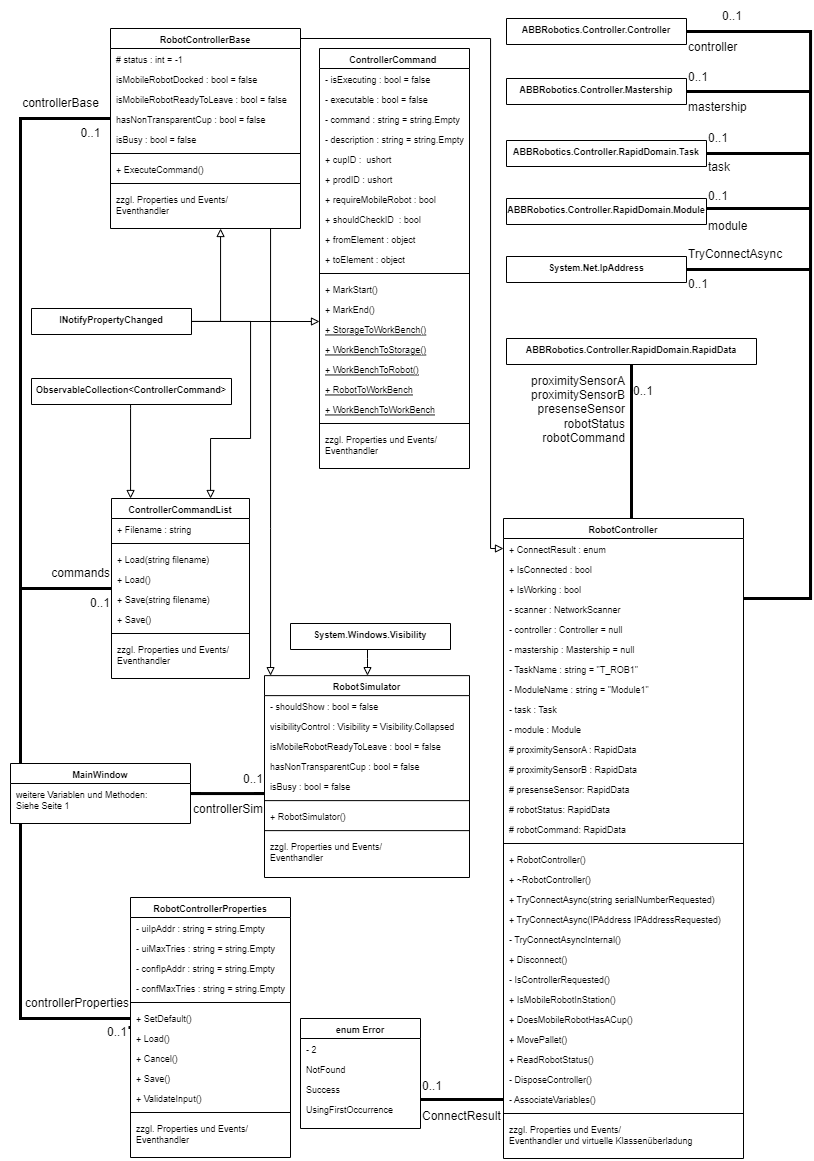
\includegraphics[width = \textwidth ]{Bilder/LV_Klassendiagramm_ABBController}
        \caption[Klassendiagramm ABB Controller ]
        {\small Klassendiagramm der MainWindow-Klasse mit Klassen aus dem ABB Controllerframework. }
        \centering
    \end{figure}

    \begin{figure}[ht]
        \label{fig:figure4}
        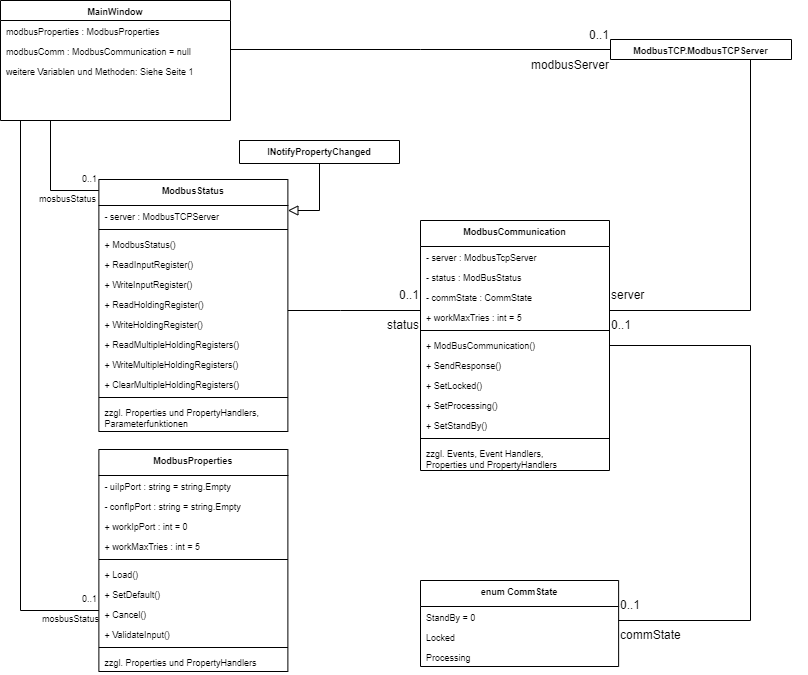
\includegraphics[width = \textwidth ]{Bilder/LV_Klassendiagramm_Modbus}
        \caption[Klassendiagramm Modbus ]
        {\small Klassendiagramm der MainWindow-Klasse mit Mosbus-Klassen }
        \centering
    \end{figure}

    \begin{figure}[ht]
        \label{fig:figure5}
        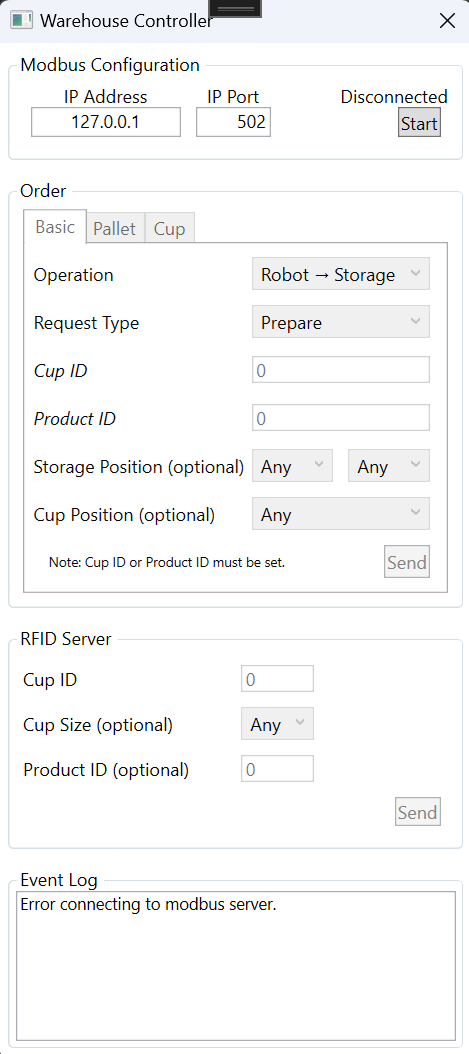
\includegraphics[height = \textheight ]{Bilder/Controller_Startbildschirm}
        \caption[Ansicht des Controller- Startbildschirm ]
        {\small Ansicht des Controller Startbildschirms. }
        \centering
    \end{figure}

    \begin{figure}[ht]
        \label{fig:figure6}
        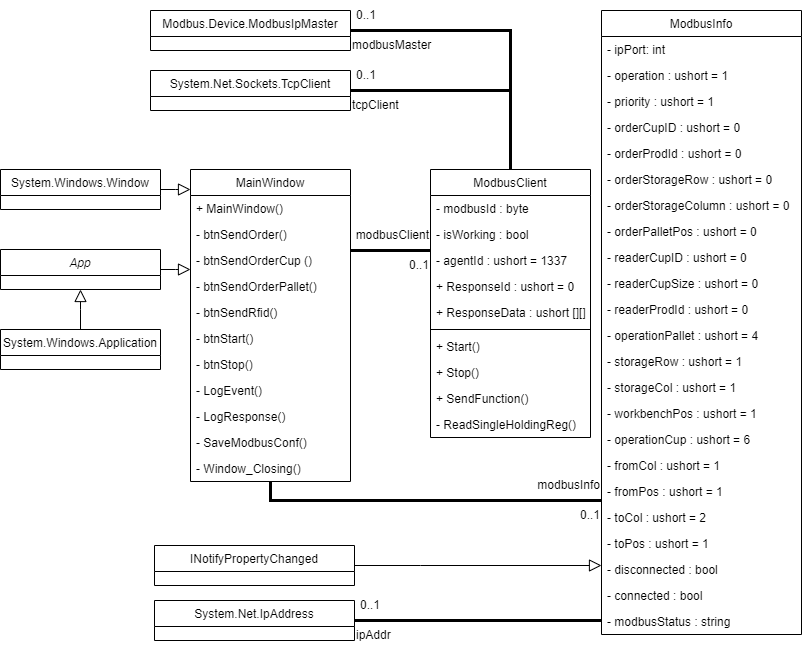
\includegraphics[width = \textwidth ]{Bilder/C_Klassendiagramm}
        \caption[Klassendiagramm des Controllers ]
        {\small Klassendiagramm des Warehouse-Controllers mit allen vererbenden Klassen jedoch ohne Klassen die
        lediglich Datentypen konvertieren.}
        \centering
    \end{figure}

    \begin{figure}[ht]
        \label{fig:figure7}
        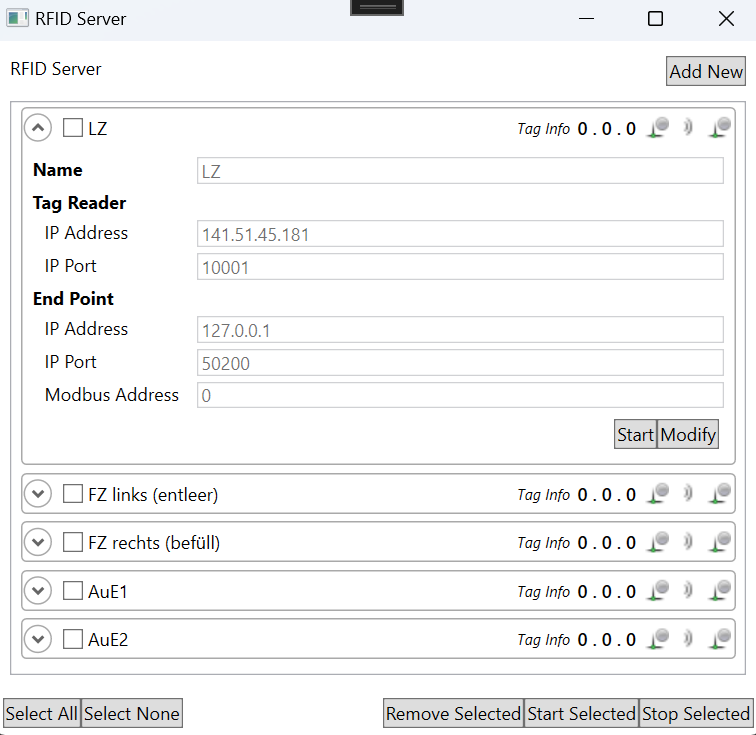
\includegraphics[height = \textwidth ]{Bilder/RFIDServer_Bildschirm}
        \caption[Startbildschirm des Programms RFID-Server]
        {\small Startbildschirm des Programms RFID-Server}
        \centering
    \end{figure}

    \begin{figure}[ht]
        \label{fig:figure8}
        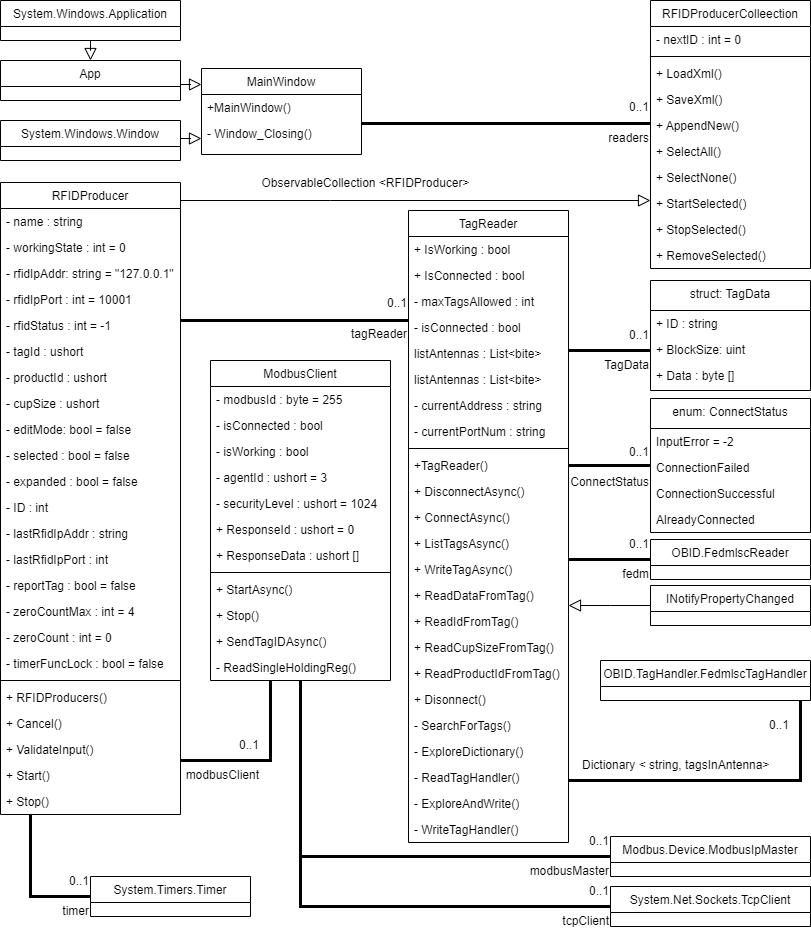
\includegraphics[width = \textwidth ]{Bilder/RFID_Klassendiagramm}
        \caption[Klassendiagramm des Programms RFID Server ]
        {\small Klassendiagramm des Programms RFID Server mit allen vererbenden Klassen jedoch ohne solche die
        lediglich Typen konvertieren.}
        \centering
    \end{figure}

    \subsection {RFID Server}

    \subsection {Controller}

